% --------------------------------------------------------------
% This is all preamble stuff that you don't have to worry about.
% Head down to where it says "Start here"
% --------------------------------------------------------------

\documentclass[12pt]{article}

\usepackage[margin=1in]{geometry} 
\usepackage{amsmath,amsthm,amssymb}
\usepackage{graphicx}
\usepackage{multirow}

\newcommand{\N}{\mathbb{N}}
\newcommand{\Z}{\mathbb{Z}}

\newenvironment{theorem}[2][Theorem]{\begin{trivlist}
		\item[\hskip \labelsep {\bfseries #1}\hskip \labelsep {\bfseries #2.}]}{\end{trivlist}}
\newenvironment{lemma}[2][Lemma]{\begin{trivlist}
		\item[\hskip \labelsep {\bfseries #1}\hskip \labelsep {\bfseries #2.}]}{\end{trivlist}}
\newenvironment{exercise}[2][Exercise]{\begin{trivlist}
		\item[\hskip \labelsep {\bfseries #1}\hskip \labelsep {\bfseries #2.}]}{\end{trivlist}}
\newenvironment{reflection}[2][Reflection]{\begin{trivlist}
		\item[\hskip \labelsep {\bfseries #1}\hskip \labelsep {\bfseries #2.}]}{\end{trivlist}}
\newenvironment{proposition}[2][Proposition]{\begin{trivlist}
		\item[\hskip \labelsep {\bfseries #1}\hskip \labelsep {\bfseries #2.}]}{\end{trivlist}}
\newenvironment{corollary}[2][Corollary]{\begin{trivlist}
		\item[\hskip \labelsep {\bfseries #1}\hskip \labelsep {\bfseries #2.}]}{\end{trivlist}}

\begin{document}
	
	% --------------------------------------------------------------
	%                         Start here
	% --------------------------------------------------------------
	
	%\renewcommand{\qedsymbol}{\filledbox}
	
	
	\title{Bike sharing demand}
	\author{Bernarda Petek\\ %replace with your name
		Mathematics with computers} %if necessary, replace with your course title
	
	\date{}
	\maketitle
	
	%\section{Abstract}
	\abstract{
		The first bike sharing system was implemented in 1965 in Netherlands. However, the project was not successful at the time, many bikes were stolen or damaged. For the next 30 years, until the early 2000s there were rarely any bike sharing systems in the world. That completely changed two decades ago with digitalization. Digitalization also made it possible to collect data about when and where the bikes are used and for how long. In this report I forecast hourly use of a Washington's bike sharing system by using and comparing different machine learning methods.
	}
	
	
	\section{Data Set}
	The data set which I am using for my project spans two years (from 2011 to 2012) usage logs of a bike sharing system in Washington, D.C., USA named Captial Bike Sharing (CBS). The data contains 12 features with types as described in the following table:
	
	\begin{center}
		\begin{tabular}{ |c|c|c| } 
			\hline
			\textbf{Name} & \textbf{Type} & \textbf{Description} \\ 
			\hline
			\hline
			count (target) & numeric & number of total rentals \\ 
			\hline
			datetime & datetime & date + hourly timestamp \\
			\hline
			season & categorical & 1 = spring, 2 = summer, 3 = fall, 4 = winter  \\ 
			\hline
			holiday & categorical & 1 = holiday, 0 = not a holiday \\ 
			\hline
			workingday & categorical & 1 = working day, 0 = not a working day \\ 
			\hline
			\multirow{4}{4em}{weather} &  & 1: Clear skies or partly cloudy \\ 
			& categorical & 2: Misty \\ 
			&  & 3: Light snowing or light raining \\ 
			&  & 4: Heavy raining or heavy snowing  \\ 
			\hline
			temp & numeric & temperature in Celsius \\ 
			\hline
			atemp & numeric & ''feels like'' temperature in Celsius \\ 
			\hline
			humidity & numeric &  relative humidity \\ 
			\hline
			windspeed & numeric &  wind speed \\  
			\hline
			casual & numeric & number of non-registered user rentals initiated \\ 
			\hline
			registered & numeric &  number of registered user rentals initiated \\ 
			\hline
			
		\end{tabular}
	\end{center}

	In my code I represent the data with \texttt{pandas} dataframe object, where every feature has its own column.
	
	\section{Preparing Data}
	The variable in which I am the most interested in is the variable \textit{count}. I am forecasting its value by testing different machine learning methods on the bike sharing data.
	
	The \textit{count} variable can be decomposed into two sub-variables: \textit{casual} and \textit{registered}, which can be summed up to produce \textit{count}. It may make sense to predict each of these two variables individually, as casual and registered users may behave differently from one another. However, for the purposes of this project, I consider only the \textit{count} variable, as it makes comparisons simpler. In the remainder of this project, I will remove the \textit{casual} and \textit{registered} variables from the analysis, as leaving them in the data frame would lead to a trivial solution, and the models would learn to predict \textit{count} simply by summing up the aforementioned variables.
	
	Instead of using variable \textit{datetime} directly I break it into few different variables. Datetime object consists of date and time measured in hours. From date I can read which day of the week it is, which I presume is important information for my machine learning models, because I suspect there are more people using bikes on certain days of the week. The same goes for month. The two newly added columns look like that: 
	
	\begin{center}
		\begin{tabular}{ |c|c|c| } 
			\hline
			\textbf{Name} & \textbf{Type} & \textbf{Description} \\ 
			\hline
			\hline
			month & categorical & 1 = January, ..., 12 = December \\ 
			\hline
			day of week & categorical & 1 = Monday, ..., 7 = Sunday \\
			\hline	
		\end{tabular}
	\end{center}

	There is one more piece of information I can get from variable \textit{datetime} and this is the time measured in hours. However, there are few different ways how the computer can interpret variable time. I take four different ways and compare them to see how their representation affect forecasting. 
	
	\subsection{Representing time}
	
	\subsubsection{Numeric representation}
	
	First and the most obvious time representation is numeric continuous representation on number line where hours are represented by natural numbers from 0 to 23 (00:00 to 23:00). This means that distance between 23:00 and 00:00 (midnight) and is the greatest which does not make that much sense because in reality midnight and 23:00 are right next to each other. This representation is found in dataframe \textit{df\_time} in consequent column.
	
		\begin{center}
		\begin{tabular}{ |c|c|c| } 
			\hline
			\textbf{Name} & \textbf{Type} & \textbf{Description} \\ 
			\hline
			\hline
			hour & numeric & hours are represented with natural numbers from 0 to 23 \\ 
			\hline	
		\end{tabular}
	\end{center}

	
	The more intuitive time representation is numeric representation with polar coordinates: $hour\_sin = \sin \varphi $, $hour\_cos = \cos \varphi$ where the value of circle radius is $r=1$ and angle $\varphi \in  [0, 2\pi]$. To get the right angle I bijectively map hour values: $$ [0, 24] \mapsto [0, 2\pi]$$. With this representation the distance between 23:00 and 00:00 is the smallest which corresponds with cyclicity of time measuring. This representation is found in dataframe \textit{df\_ctime} in consequent columns: 
	
	\begin{center}
		\begin{tabular}{ |c|c|c| } 
			\hline
			\textbf{Name} & \textbf{Type} & \textbf{Description} \\ 
			\hline
			\hline
			hour\_sin & numeric & x-axis polar coordinate \\ 
			\hline	
			hour\_cos & numeric & y-axis polar coordinate \\ 
			\hline
		\end{tabular}
	\end{center}
	
	\subsubsection{Categorical representation}
	
	Time can also be represented as a categorical variable with 24 different categories because its value is integer from interval $[0, 24]$. This is my third representation which is found in dataframe \textit{df\_dtime24} in consequent column:  
	
	\begin{center}
		\begin{tabular}{ |c|c|c| } 
			\hline
			\textbf{Name} & \textbf{Type} & \textbf{Description} \\ 
			\hline
			\hline
			hour & categorical & hours are represented with natural numbers from 0 to 23 \\ 
			\hline	
		\end{tabular}
	\end{center}
	
	
	\begin{figure}
		\centering
		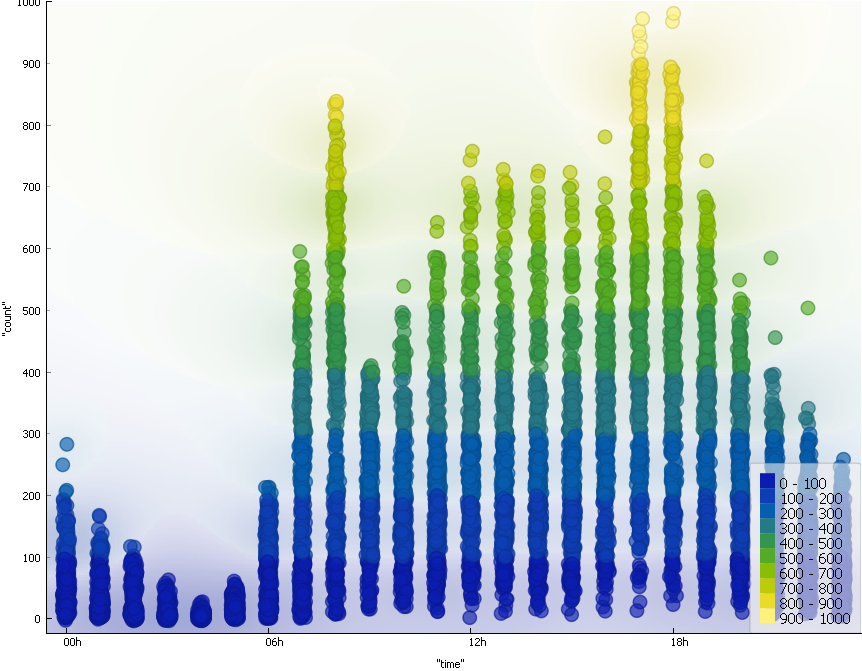
\includegraphics[scale=0.4] {graf}
		\caption{\label{fig:1} A visualization of the bikes in use in its relation to time of day. The plot clearly indicates hourly trends, showing that bike demand goes up around 8:00 and 16:00.}
	\end{figure}
	
	Distribution of hourly use of bikes which can be seen on Figure \ref{fig:1} is the motivation behind my last representation of the time. Time is again represented as a categorical variable, only this time I use different categories. I use seven different categories: $[$1:00, 2:00, 3:00, 4:00, 5:00, 6:00$]$, $[$7:00, 8:00$]$, $[$9:00, 10:00$]$, $[$11:00, 12:00, 13:00, 14:00, 15:00, 16:00$]$, $[$17:00, 18:00$]$, $[$19:00, 20:00$]$, $[$21:00, 22:00, 23.00, 00:00$]$. The last time representation is found in dataframe \textit{df\_dtime\_categ} in consequent column:
	
	\begin{center}
		\begin{tabular}{ |c|c|c| } 
			\hline
			\textbf{Name} & \textbf{Type} & \textbf{Description} \\ 
			\hline
			\hline
			hour & categorical & hours are represented with natural numbers from 1 to 7 \\ 
			\hline	
		\end{tabular}
	\end{center}
			
			
	\section{Processing Data}
	
	\subsection{One hot encoding}
	
	There are many different ways one can treat categorical variables so that machine learning algorithms can read them as they are - categories. One of the most popular way is one hot encoding. One hot encoding is a process which transforms categorical variables into a form that helps machine learning algorithms understand the categorical nature of these variables. One hot encoding breaks categorical variable's column into $n$ different columns, where $n$ is the number of categories. Values in individual column are $0$ if categorical value does not correspod with column's category or $1$ if it does. This allows a machine learning model to uniquely determine each row's category by finding the entry with the value $1$.
	
	There are many categorical variables in my data. I use one hot encoding on all of them, let's take a look at variable named \textit{season}. \textit{Season} is a categorical variable with 4 different categories: spring, summer, fall, winter. Season column is broken into 4 different columns in the same way as it is shown in an example:
	
	\begin{center}
		\begin{tabular}{ |c|c|c|c|c|  } 
			\hline
			\textbf{Season} & \textbf{Spring} & \textbf{Summer} & \textbf{Autumn} & \textbf{Winter} \\
			\hline
			\hline
			summer & 0 & 1 & 0 & 0 \\
			\hline
			spring & 1 & 0 & 0 & 0 \\
			\hline
			winter & 0 & 0 & 0 & 1 \\
			\hline
			summer & 0 & 1 & 0 & 0 \\
			\hline
			autumn & 0 & 0 & 1 & 0 \\
			\hline
			spring & 1 & 0 & 0 & 0 \\
			\hline
		\end{tabular}
	\end{center}

	However, when using one hot encoding, there are usually $n-1$ columns, because the computer understands option where there are only zeros in a row as a $n$-th category.
	
	\subsection{Standardization}
	
	Standardization is the process of changing the values of variables so that their variance is $1$ and their mean is 0. The goal for all variables is to have the same scale without changing their relations and range of values. Before forecasting I standardize all dataframes.
	
	\section{Forecasting}
	
	For forecasting I am using cross-validation with ten different machine learning algorithms, some of which I programmed it from stratch, on the four variants of  data sets. 
	
	\subsection{Cross-validation}
	Cross-validation is a widely used machine learning technique that uses different parts of data to train and test machine learning model on different iterations. I am using 5-fold cross-validation.
	
	The data is partitioned into $k$ equal sets. $k-1$ sets are training sets and the remaining one is a testing set. There are $k$ iterations and each of the $k$ equal sets is a testing set exactly once. Final result is the mean value of all $k$ forecastings on $k$ testing sets.
	
	\subsection{ML algorithms}
	I am using the following machine learning models:
	\begin{itemize}
		\item Ridge Regression
		\item Decision Trees
		\item Random Forest
		\item Gradient Boosting
		\item Neural Network
		\item Support Vector Regression
		\item K-Nearest Neighbour
		\item Bagging with Ridge Regression
		\item Bagging with K-Nearest Neighbour
		\item Bagging with Decision Trees
	\end{itemize}
	\subsection{Computing the error}
	
	\subsubsection{RMSE}
		The root-mean-squared error is a commonly used metric for evaluating the quality of machine learning models in regression tasks. It's function is to compare the predicted values of the machine learning models and the true values. Its formula is: 
		
		$$\text{RMSE} = \sqrt{\frac{\Sigma_{i=1}^{n} (x_i-y_i)^2}{n}}$$
		
		where $n$ is number of points in testing data, $x=(x_1, x_2, ..., x_n)$ is the testing data and $y=(y_1, y_2, ..., y_n)$ are the forecasting results for the testing data.
		
	\subsubsection{Error ratio}
	
	Even though the RMSE is one of the most commonly used metrics when evaluating regression tasks, it is difficult to determine how good the models are by looking at this number alone. We can compare the models amongst each other and pick the one with the lowest RMSE. However, it may make more intuitive sense to present the results in the improvement in predictions over a naive model, e.g. a mean prediction. We call this metric the error ratio. We compute the error ratio by taking the ratio between the naive mean prediction, which ignores all the variables in the data set, and compare it to the error produced by our machine learning models. This gives us a better understanding of how well our model is actually performing because it tells us how much we've managed to reduce the error from when doing the simplest possible thing.
	
	\subsection{Evaluating the results}
	The results are shown in the tables below. 
	
	\begin{center}
		\begin{tabular}{ |c|c|c|c|c|  } 
			\hline
			\textbf{RMSE} & df\_time & df\_ctime & df\_dtime24 & df\_dtime\_categ \\
			\hline
			Ridge Regression & 145.53 & 134.1 & 109.48 & 115.03 \\
			Decision Trees & 90.12 & 90.83 & 105.21 & 106.1 \\
			Random Forest & \textbf{66.26} & \textbf{66.75} & 76.39 & \textbf{78.98} \\
			Gradient Boosting & 82.34 & 82.68 & 91.71 & 89.27 \\
			Neural Network & 389.74 & 98.7 &\textbf{ 70.14} & 83.23 \\
			Support Vector Regression & 161.8 & 152.76 & 149.95 & 149.95 \\
			K-Nearest Neighbour & 139.95 & 120.23 & 93.42 & 99.28 \\
			Bagging with Ridge Regression & 145.51 & 134.09 & 109.47 & 115.05 \\
			Bagging with K-Nearest Neighbour & 143.69 & 128.88 & 98.82 & 111.07 \\
			Bagging with Decision Trees & \textbf{65.96} &\textbf{ 66.94} & \textbf{76.38} & \textbf{78.32} \\
			\hline
		\end{tabular}
	\end{center}

\begin{center}
	\begin{tabular}{ |c|c|c|c|c|  } 
		\hline
		\textbf{RMSE RATIO} & df\_time & df\_ctime & df\_dtime24 & df\_dtime\_categ \\
		\hline
		Ridge Regression & 0.8 & 0.74 & 0.6 & 0.64 \\
		Decision Trees & 0.5 & 0.5 & 0.58 & 0.59 \\
		Random Forest & \textbf{0.37} & \textbf{0.37} & 0.42 & \textbf{0.44} \\
		Gradient Boosting & 0.45 & 0.46 & 0.51 & 0.49 \\
		Neural Network & 2.15 & 0.54 &\textbf{ 0.39} & 0.46 \\
		Support Vector Regression & 0.89 & 0.84 & 0.83 & 0.83 \\
		K-Nearest Neighbour & 0.77 & 0.66 & 0.52 & 0.55 \\
		Bagging with Ridge Regression & 0.8 & 0.74 & 0.6 & 0.64 \\
		Bagging with K-Nearest Neighbour & 0.79 & 0.71 & 0.55 & 0.61 \\
		Bagging with Decision Trees & \textbf{0.36} & \textbf{0.37} & 0.42 & \textbf{0.43} \\
		\hline
	\end{tabular}
\end{center}
	
	
	\section{Conclusion}
	The best algorithm was almost always Random Forest algorithm, which is not unusual because it is a very robust algorithm. We can also see that from the fact that it did not matter how the time variable was represented, the results were not far from each other when using Random Forest algorithm. However, it needs quite a lot computational power. It is not unusual that Bagging with Decision Trees gives the same result as Random Forest, because these two algorithms are basically the same. The most interesting thing is that there are some algorithms where the difference between different representations of time variable is very apparent. For example, Neural Network algorithm worked the worst by far when time was continuos but not cyclic. In most cases algorithms worked better when time variable was categorical. The reason for that can be seen on Figure \ref{fig:1}
	
	
	
	
	% --------------------------------------------------------------
	%     You don't have to mess with anything below this line.
	% --------------------------------------------------------------
	
	
\end{document}